\section{\large \textcolor{blue}{Óptica geométrica}}

\begin{flushleft}
\textbf{\textcolor{blue}{\Large Quest\~ao - Entrada da Fibra Óptica — Lei de Snell}}\\
\noindent

\subsection{Quest\~ao Entrada da Fibra Óptica — Lei de Snell}

\vspace{0.5cm}

\textcolor{red}{\textbf{Solução:}}\\

\section*{Índices de Refração}

\begin{itemize}
    \item $n_1 = 1$
    \item $n_2 = 1{,}6$
    \item $n_3 = 1{,}5$
\end{itemize}

\section*{Entrada da Fibra Óptica (Raio de Luz)}

Utilizando a \textbf{Lei de Snell}, temos:

\subsection*{1. Incidência do meio $n_1$ para o meio $n_2$ (ponto 1):}
\[
n_1 \cdot \sin \theta = n_2 \cdot \sin \phi
\Rightarrow \sin \theta = 1{,}6 \cdot \sin \phi
\]

\subsection*{2. Reflexão Total Interna no ponto (2):}
\[
n_2 \cdot \sin \alpha = n_3 \cdot \sin 90^\circ
\Rightarrow 1{,}6 \cdot \sin \alpha = 1{,}5 \cdot 1 = 1{,}5
\Rightarrow \sin \alpha = \frac{1{,}5}{1{,}6}
\]

\subsection*{3. Substituindo na equação de Snell:}
\[
\sin \theta = 1{,}6 \cdot \sin \phi
\qquad
\text{e}
\qquad
\sin \alpha = \frac{1{,}5}{1{,}6} = \frac{15}{16}
\]

\subsection*{4. Cálculo de $\sin \theta$:}
\[
\sin \theta = 1{,}6 \cdot \sin \phi = \frac{15}{10} = \frac{3{,}5}{4{,}4}
\]

\section*{Identidade Trigonométrica (para reflexão total):}

Sabemos que:
\[
\phi + \alpha = 90^\circ
\Rightarrow \alpha = 90^\circ - \phi
\]

Portanto:
\[
\sin (90^\circ - \phi) = \cos \phi
\quad \Rightarrow \quad
\sin \alpha = \cos \phi
\]

Logo:
\[
\sin(90^\circ - \phi) = \sin 90^\circ \cdot \cos \phi - \cos 90^\circ \cdot \sin \phi = \cos \phi
\]

Sabemos que:

\[
\cos \phi = \frac{15}{16}
\]

Pelo fato de que:
\[
\sin^2 \phi + \cos^2 \phi = 1
\Rightarrow \sin^2 \phi = 1 - \left(\frac{15}{16}\right)^2
= \frac{256 - 225}{256} = \frac{31}{256}
\]

\[
\Rightarrow \sin \phi = \sqrt{\frac{31}{256}}
\]

Agora, usando a equação:
\[
\sin \theta = 1{,}6 \cdot \sin \phi
\Rightarrow \sin \theta = 1{,}6 \cdot \sqrt{\frac{31}{256}}
= \frac{16}{10} \cdot \sqrt{\frac{31}{256}}
= \frac{16}{10} \cdot \frac{\sqrt{31}}{16}
= \frac{\sqrt{31}}{10}
\]

Portanto, o ângulo de incidência máximo é:

\[
\boxed{
\theta = \sin^{-1} \left( \frac{\sqrt{31}}{10} \right)
}
\]

\end{flushleft}


\begin{flushleft}
\textbf{\textcolor{blue}{\Large Quest\~ao 23 - IFFAR 2023 - Associa\c{c}\~ao de Lentes Delgadas}}\\
\noindent

\subsection{Quest\~ao 23 - IFFAR 2023 - Associa\c{c}\~ao de Lentes Delgadas}

Sistemas \'opticos compostos por associa\c{c}\~ao de lentes desempenham um papel fundamental no ensino de f\'isica no campo da \'optica geom\'etrica. Eles s\~ao utilizados para produzir imagens com caracter\'isticas especiais, assim como aquelas obtidas por microsc\'opios compostos ou lunetas astron\^omicas.

Nesse contexto, considere um caso te\'orico em que duas lentes delgadas, sendo elas coaxiais, s\~ao associadas com uma dist\^ancia $d = 15\,cm$ entre elas. As lentes t\^em dist\^ancias focais $f_1 = 10\,cm$ e $f_2 = 2\,cm$.

Qual \'e a verg\^encia equivalente da associa\c{c}\~ao das lentes?

\begin{itemize}
\item[(A)] $-0{,}07\,di$
\item[(B)] $-15\,di$
\item[(C)] $0{,}02\,di$
\item[(D)] $12\,di$
\item[(E)] $60\,di$
\end{itemize}

\vspace{0.5cm}

\begin{center}
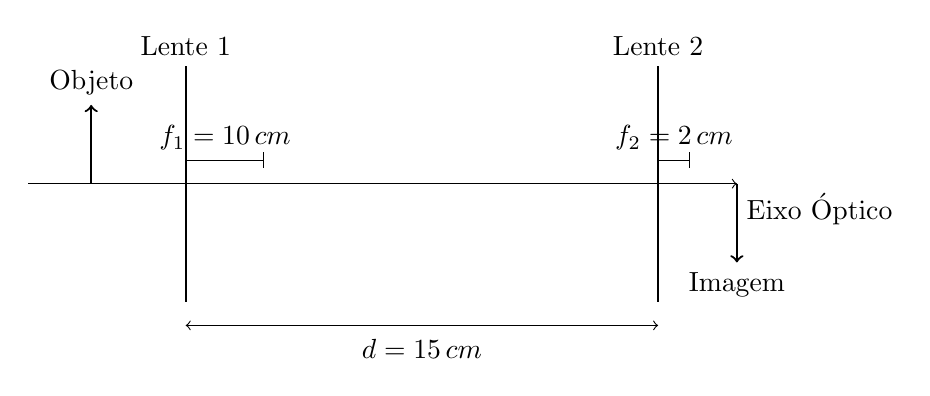
\begin{tikzpicture}[scale=1]

% Eixo principal
\draw[->] (-2,0) -- (7,0) node[below right] {Eixo Óptico};

% Lentes
\draw[thick] (0,-1.5) -- (0,1.5);
\draw[thick] (6,-1.5) -- (6,1.5);

% Rótulos das lentes
\node[above] at (0,1.5) {Lente 1};
\node[above] at (6,1.5) {Lente 2};

% Distância entre lentes
\draw[<->] (0,-1.8) -- (6,-1.8);
\node at (3,-2.1) {$d = 15\,cm$};

% Foco da lente 1 (esquerda)
\draw[|-|] (0,0.3) -- (1,0.3);
\node[above] at (0.5,0.3) {$f_1 = 10\,cm$};

% Foco da lente 2 (direita)
\draw[|-|] (6,0.3) -- (6.4,0.3);
\node[above] at (6.2,0.3) {$f_2 = 2\,cm$};

% Objeto
\draw[->, thick] (-1.2,0) -- (-1.2,1);
\node[above] at (-1.2,1) {Objeto};

% Imagem final (só referência)
\draw[->, thick] (7,0) -- (7,-1);
\node[below] at (7,-1) {Imagem};

\end{tikzpicture}
\end{center}

\textcolor{red}{\textbf{Solu\c{c}\~ao:}}\\

Quando duas lentes delgadas s\~ao associadas a uma certa dist\^ancia $d$ entre si, a verg\^encia equivalente do sistema \'optico \'{e} dada por:

\[
\boxed{
V = V_1 + V_2 - d \cdot V_1 \cdot V_2
}
\]

Onde:
\begin{itemize}
    \item $V_1 = \dfrac{100}{f_1}$, com $f_1$ em cm
    \item $V_2 = \dfrac{100}{f_2}$, com $f_2$ em cm
    \item $d$ \'e a dist\^ancia entre as lentes, em metros
\end{itemize}

Calculamos as verg\^encias individuais:

\[
V_1 = \frac{100}{10} = 10\,di
\qquad
V_2 = \frac{100}{2} = 50\,di
\]

Convertendo a dist\^ancia $d$ para metros:

\[
d = 15\,cm = 0{,}15\,m
\]

Substituindo na f\'ormula da verg\^encia equivalente:

\[
V = 10 + 50 - 0{,}15 \cdot 10 \cdot 50
\]

\[
V = 60 - 0{,}15 \cdot 500 = 60 - 75 = -15\,di
\]

\vspace{0.3cm}

Portanto, a resposta correta \'e a alternativa \colorbox{green!50}{\textbf{B)}}.

\end{flushleft}


\begin{flushleft}

\textbf{\textcolor{blue}{\Large Vis\~ao de Cores}}\\
\noindent

A vis\~ao de cores ocorre por meio da intera\c{c}\~ao da luz com c\'elulas fotorreceptoras localizadas na \textbf{retina}, 
denominadas \textbf{cones}. Esses receptores s\~ao sens\'iveis a diferentes \textbf{comprimentos de onda} da luz vis\'ivel, 
permitindo a percep\c{c}\~ao das cores.

\begin{itemize}
    \item \textbf{Passo 1: Entrada da luz} - A luz refletida pelos objetos penetra no olho atrav\'es da \textbf{c\'ornea}, 
    passando pela \textbf{pupila} e sendo focalizada pelo \textbf{cristalino}.
    \item \textbf{Passo 2: Chegada \`a retina} - A luz atinge a \textbf{retina}, onde se localizam os cones (vis\~ao colorida) 
    e bastonetes (vis\~ao em preto e branco).
    \item \textbf{Passo 3: Tipos de cones} - Existem tr\^es tipos principais:
    \begin{itemize}
        \item Cones S - sens\'iveis \`a luz azul-violeta ($\approx 420\,\text{nm}$).
        \item Cones M - sens\'iveis \`a luz verde ($\approx 530\,\text{nm}$).
        \item Cones L - sens\'iveis \`a luz vermelho-alaranjada ($\approx 560\,\text{nm}$).
    \end{itemize}
    \item \textbf{Passo 4: Combina\c{c}\~ao de sinais} - A percep\c{c}\~ao de cores decorre da ativa\c{c}\~ao combinada dos diferentes 
    tipos de cones (\textit{teoria tricrom\'atica}).
    \item \textbf{Passo 5: Processamento neural} - Os impulsos el\'etricos gerados s\~ao transmitidos pelo \textbf{nervo \'optico} at\'e 
    o \textbf{c\'ortex visual} no lobo occipital, onde ocorre a interpreta\c{c}\~ao final da cor percebida.
\end{itemize}

\textbf{Resumo:} A vis\~ao de cores depende dos cones da retina, cada tipo especializado em uma faixa de comprimentos de onda. A combina\c{c}\~ao das respostas desses cones permite ao c\'erebro diferenciar milh\~oes de tonalidades.


\textbf{\textcolor{blue}{\Large Quest\~ao - 37 IFSC 2023 - Refração de Luz}}\\
\noindent

\subsection{Quest\~ao - 37 IFSC 2023 - Refração de Luz}
A vis\~ao das cores \'e um processo complexo que envolve diferentes tipos de c\'elulas fotossens\'iveis presentes na retina. 
A luz atravessa diferentes estruturas presentes no olho at\'e atingir os cones e os bastonetes, que s\~ao respons\'aveis pela 
detec\c{c}\~ao de est\'imulos luminosos e desempenham pap\'eis distintos na percep\c{c}\~ao visual. Com base nesse contexto, 
analise as assertivas abaixo e assinale \textbf{V}, se verdadeiras, ou \textbf{F}, se falsas.

\begin{enumerate}
\item ( \ \ ) Os cones s\~ao respons\'aveis pela vis\~ao em cores, diferenciando diferentes frequ\^encias da luz, e s\~ao mais sens\'iveis a 
altas amplitudes da onda luminosa.
\item ( \ \ ) Os bastonetes s\~ao respons\'aveis pela vis\~ao em preto e branco e s\~ao mais sens\'iveis a altas amplitudes da onda luminosa.
\item ( \ \ ) Os cones s\~ao respons\'aveis pela vis\~ao em preto e branco, diferenciando diferentes amplitudes da onda luminosa, e s\~ao mais 
sens\'iveis a baixas frequ\^encias da luz.
\item ( \ \ ) Ap\'os atravessar a pupila, a luz passa pelas seguintes estruturas, em ordem, do olho at\'e atingir a retina: C\'ornea, Humor 
Aquoso, Cristalino e Humor V\'itreo.
\end{enumerate}

A ordem correta de preenchimento dos par\^enteses, de cima para baixo, \'e:
\begin{itemize}
\item[(A)] V - F - F - F.
\item[(B)] V - V - F - V.
\item[(C)] F - F - V - F.
\item[(D)] V - F - F - V.
\item[(E)] F - V - V - F.
\end{itemize}

\vspace{0.5cm}

\textcolor{red}{\textbf{Solução:}}\\

\textbf{Análise das assertivas:}
\begin{itemize}
    \item[(1)] \textbf{Verdadeira.} Os \textbf{cones} s\~ao c\'elulas fotorreceptoras especializadas na percep\c{c}\~ao das \textbf{cores}, sens\'iveis a diferentes \textbf{frequ\^encias} da luz (curta, m\'edia e longa), funcionando melhor sob alta intensidade luminosa (maior amplitude de onda luminosa).
    
    \item[(2)] \textbf{Falsa.} Os \textbf{bastonetes} s\~ao respons\'aveis pela vis\~ao em preto e branco, mas atuam em condi\c{c}\~oes de \textbf{baixa intensidade luminosa}, sendo muito sens\'iveis a pequenas amplitudes da onda luminosa.
    
    \item[(3)] \textbf{Falsa.} Os cones n\~ao s\~ao respons\'aveis pela vis\~ao em preto e branco, mas sim pela vis\~ao colorida. A vis\~ao monocrom\'atica est\'a relacionada aos bastonetes.
    
    \item[(4)] \textbf{Falsa.} A ordem apresentada est\'a incorreta, pois a \textbf{c\'ornea} vem antes da pupila. O caminho correto da luz at\'e a retina \'e: \textbf{C\'ornea} $\rightarrow$ \textbf{Humor Aquoso} $\rightarrow$ \textbf{Pupila} $\rightarrow$ \textbf{Cristalino} $\rightarrow$ \textbf{Humor V\'itreo} $\rightarrow$ \textbf{Retina}.
\end{itemize}

\textbf{Sequ\^encia correta:} \colorbox{green!50}{\textbf{V - F - F - F}}.

A alternativa correta \'e: \colorbox{green!50}{\textbf{A}}.

\end{flushleft}

\begin{flushleft}
\textbf{\textcolor{blue}{\Large Quest\~ao 43 - IFSC 2023 - Associação de Lentes}}\\
\noindent

\subsection{Quest\~ao 43 - IFSC 2023 - Associação de Lentes}
A associa\c{c}\~ao de lentes \'e frequentemente utilizada para obter caracter\'isticas espec\'ificas na imagem final de um objeto, como \'e o caso da luneta 
astron\^omica e do microsc\'opio composto. Na Figura 6, temos uma representa\c{c}\~ao de uma associa\c{c}\~ao entre uma lente convergente delgada com 
dist\^ancia focal $f_1=10\ \mathrm{cm}$ e uma lente divergente tamb\'em delgada com dist\^ancia focal $f_2=20\ \mathrm{cm}$, separadas por uma dist\^ancia 
de $5\ \mathrm{cm}$.

\begin{figure}
    \centering
    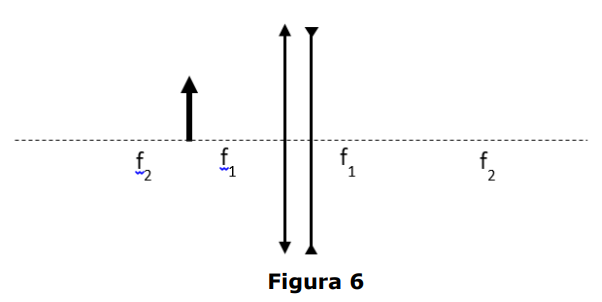
\includegraphics[width=0.5\textwidth]{figures/associacao-de-lentes.png}
\end{figure}

Ao posicionar um objeto a uma dist\^ancia de $12\ \mathrm{cm}$ \`a esquerda da lente convergente, a imagem final observada por um observador \`a direita da lente divergente ter\'a as seguintes caracter\'isticas:

\begin{itemize}
  \item[(A)] Imagem real, direta e maior.
  \item[(B)] Imagem virtual, invertida e menor.
  \item[(C)] Imagem virtual, direta e igual.
  \item[(D)] Imagem real, invertida e menor.
  \item[(E)] Imagem real, invertida e maior.
\end{itemize}

\vspace{0.5cm}

\textcolor{red}{\textbf{Solu\c{c}\~ao detalhada:}}\\

\textbf{1) Escolha do referencial e posi\c{c}\~oes} \\
Para resolver com clareza, posicionamos as lentes ao longo do eixo $x$ da seguinte forma (escolha consistente com a figura e o enunciado): a lente divergente (L$_2$) em $x=0$ e a lente convergente (L$_1$) em $x=+5\ \mathrm{cm}$. Assim, o objeto (que est\'a $12\ \mathrm{cm}$ \`a esquerda de L$_1$) fica em
\[
x_{\text{obj}}=x_{L_1}-12=5-12=-7\ \mathrm{cm}.
\]
Usaremos a conven\c{c}\~ao de lentes delgadas: dist\^ancias de objeto $d_o$ medidas positivamente \`a esquerda da lente, dist\^ancias de imagem $d_i$ positivas \`a direita da lente; $f>0$ para convergente e $f<0$ para divergente.

\medskip

\textbf{2) Primeira lente (L$_2$ -- divergente, $f_2=-20\ \mathrm{cm}$)} \\
Dist\^ancia objeto relativa a L$_2$:
\[
d_{o2}=x_{L_2}-x_{\text{obj}}=0-(-7)=7\ \mathrm{cm}.
\]
Equa\c{c}\~ao das lentes delgadas:
\[
\frac{1}{f_2}=\frac{1}{d_{o2}}+\frac{1}{d_{i2}}
\quad\Rightarrow\quad
\frac{1}{d_{i2}}=\frac{1}{f_2}-\frac{1}{d_{o2}}
=\frac{1}{-20}-\frac{1}{7}=-\frac{27}{140}.
\]
Logo
\[
d_{i2}=-\frac{140}{27}\ \mathrm{cm}\approx -5{,}185\ \mathrm{cm}.
\]
O sinal negativo indica que a imagem (I$_2$) formada por L$_2$ est\'a \`a \textbf{esquerda} de L$_2$ (imagem virtual relativa a L$_2$), em
\[
x_{I_2}=x_{L_2}+d_{i2}=0-\frac{140}{27}=-\frac{140}{27}\ \mathrm{cm}\approx -5{,}185\ \mathrm{cm}.
\]
A amplia\c{c}\~ao da L$_2$ \'e
\[
m_2=-\frac{d_{i2}}{d_{o2}}=-\frac{-140/27}{7}=\frac{140}{189}=\frac{20}{27}\approx 0{,}74074.
\]
(I$_2$ \'e direita/mesmo sentido que o objeto original porque $m_2>0$.)

\medskip

\textbf{3) Segunda lente (L$_1$ -- convergente, $f_1=10\ \mathrm{cm}$)} \\
A imagem I$_2$ formada por L$_2$ passa a ser o objeto para L$_1$. A dist\^ancia objeto para L$_1$ \'e
\[
d_{o1}=x_{L_1}-x_{I_2}=5-\Big(-\frac{140}{27}\Big)=\frac{275}{27}\ \mathrm{cm}\approx 10{,}185\ \mathrm{cm}.
\]
Aplicando a f\'ormula da lente:
\[
\frac{1}{d_{i1}}=\frac{1}{f_1}-\frac{1}{d_{o1}}
=\frac{1}{10}-\frac{27}{275}=\frac{275-270}{2750}=\frac{1}{550}.
\]
Portanto
\[
d_{i1}=550\ \mathrm{cm}.
\]
O sinal positivo indica que a imagem final (I$_1$) est\'a \`a \textbf{direita} de L$_1$ (imagem \textbf{real}), em
\[
x_{I_1}=x_{L_1}+d_{i1}=5+550=555\ \mathrm{cm}.
\]
A amplia\c{c}\~ao da L$_1$ \'e
\[
m_1=-\frac{d_{i1}}{d_{o1}}
=-\frac{550}{275/27}=-54.
\]

\medskip

\textbf{4) Amplitude total e orienta\c{c}\~ao da imagem final} \\
A amplia\c{c}\~ao total do sistema \'e
\[
m_{\text{total}}=m_1\cdot m_2
=(-54)\cdot\frac{20}{27}=-40.
\]
O sinal negativo indica que a imagem final est\'a \textbf{invertida} em rela\c{c}\~ao ao objeto original; o valor absoluto $|m_{\text{total}}|=40$ significa que a imagem \'e \textbf{muito maior} que o objeto (amplitude linear 40 vezes).

\medskip

\textbf{5) Conclus\~ao} \\
A imagem final observada por um observador \`a direita da lente divergente \'e:
\begin{itemize}
  \item \textbf{real} (pois $d_{i1}=550\ \mathrm{cm}>0$),
  \item \textbf{invertida} (pois $m_{\text{total}}<0$),
  \item \textbf{maior} (pois $|m_{\text{total}}|=40>1$).
\end{itemize}

Portanto, a alternativa correta \'e: \colorbox{green!50}{\textbf{E}}.

\end{flushleft}



\begin{flushleft}
\textbf{\textcolor{blue}{\Large Quest\~ao - }}\\
\noindent

\subsection{Quest\~ao }

\begin{itemize}
\item[(A)] 
\item[(B)] 
\item[(C)]
\item[(D)] 
\item[(E)] 
\end{itemize}

\vspace{0.5cm}

\textcolor{red}{\textbf{Solução:}}\\


A resposta correta é alternativa \colorbox{green!50}{\textbf{...}}.

\end{flushleft}




